\documentclass[12pt]{article}
\usepackage[utf8]{inputenc}
\usepackage{graphicx}    % For figures
\usepackage{float}       % Force figure placement with [H]
\usepackage{amsmath}     % For math symbols
\usepackage{geometry}    % For margin control
\usepackage{caption}     % For better captions
\usepackage{hyperref}    % For hyperlinks
\usepackage{booktabs}    % For clean tables
\geometry{margin=1in}

\title{Unsupervised Learning - Final Project}
\author{Isaac Benadiba , Yuval Ramot }

\begin{document}

\maketitle

\begin{abstract}
This project explores the application of unsupervised learning techniques to uncover latent structure in wine data based solely on chemical properties. Without relying on any labels or external annotations, we aim to identify natural groupings of wines, detect anomalies, and interpret the underlying geometry of the dataset.

We begin by standardizing the data and applying Principal Component Analysis (PCA) to reduce its dimensionality. Clustering is then performed using K-Means, DBSCAN, and Gaussian Mixture Models (GMM), each offering a different view of the data’s organization: centroid-based, density-based, and probabilistic. We determine the optimal number of clusters using the elbow method and validate clustering performance through the silhouette score. A t-distributed Stochastic Neighbor Embedding (t-SNE) visualization is used to illustrate the separation between clusters in a non-linear projection.

Our results show that both K-Means and GMM achieve high silhouette scores (0.5119 and 0.5140 respectively), while DBSCAN provides a complementary structure with the added benefit of identifying outliers. Anomaly detection is performed using DBSCAN’s noise points and low-likelihood samples from GMM, capturing distinct sets of rare wines. Statistical tests including one-way ANOVA and paired t-tests confirm that the performance differences across models are significant.

Overall, the analysis demonstrates that unsupervised learning can reveal meaningful wine archetypes and detect unusual samples without any prior labeling. The combination of visual, statistical, and algorithmic tools provides a robust pipeline for exploring hidden structure in complex datasets.
The code is available at  %--------git--------- 
\end{abstract}


\section{Introduction}

Unsupervised learning is a core area of machine learning that focuses on discovering hidden patterns, structures, or groupings within unlabeled data. Unlike supervised learning, which relies on labeled examples, unsupervised methods aim to find meaningful organization in data without any prior annotations. This makes them especially valuable in exploratory data analysis, where no ground truth is available.

In this project, we investigate whether unsupervised learning algorithms can reveal latent structure in a real-world dataset of wines. Specifically, we aim to identify natural groupings — or "archetypes" — of wine based solely on their chemical properties, without access to quality labels or human-crafted categories. We explore whether the chemical composition of wine is sufficient to distinguish styles or profiles, and whether different algorithms converge on similar clusterings.

To do this, we apply three fundamental techniques in unsupervised learning: clustering, dimensionality reduction, and anomaly detection.
\textbf{Clustering} involves partitioning data points into groups such that members of the same group are more similar to each other than to those in other groups. \textbf{Dimensionality reduction} transforms high-dimensional data into a lower-dimensional representation, preserving the most important structure while enabling visualization and reducing computational complexity. 
\textbf{Anomaly detection} seeks to identify samples that deviate significantly from the norm — these outliers may represent rare or unusual patterns in the data.

We apply these techniques to a dataset of wine samples described by 11 chemical attributes. After standardizing the features, we perform Principal Component Analysis (PCA) for dimensionality reduction, followed by clustering using K-Means, DBSCAN, and Gaussian Mixture Models (GMM). We evaluate clustering quality using the silhouette score and validate our findings with statistical tests including ANOVA and paired t-tests. For anomaly detection, we compare results from DBSCAN and GMM-based likelihood methods. Finally, we use t-SNE for non-linear visualization of the clustering structure, providing intuitive insights into the discovered groupings.

This analysis demonstrates how unsupervised learning can uncover latent structure in real-world data, even in the absence of labeled outcomes. The project emphasizes both interpretability and statistical rigor, combining visual and quantitative methods to support every claim.


\section{Methods}

\subsection*{Data Description}
We used the Wine Quality dataset from Kaggle\footnote{\url{https://www.kaggle.com/datasets/taweilo/wine-quality-dataset-balanced-classification}}, containing 11 numerical chemical features. The quality label was removed to ensure a fully unsupervised setting.

\subsection*{Data Preprocessing}
All features were standardized using Scikit-learn’s \texttt{StandardScaler}, ensuring zero mean and unit variance. The scaled data was used throughout the analysis.

\subsection*{Dimensionality Reduction}
We applied Principal Component Analysis (PCA) to reduce dimensionality for visualization and clustering. The first two principal components were retained. PCA was also used to initialize t-SNE for non-linear projection.

\subsection*{Clustering Algorithms}
We applied three clustering algorithms:
\begin{itemize}
    \item \textbf{K-Means}: using the elbow method to determine $K=3$.
    \item \textbf{DBSCAN}: parameters chosen using a k-distance graph ($\epsilon = 0.17$, \texttt{min\_samples} = 5).
    \item \textbf{Gaussian Mixture Models (GMM)}: with three components to match K-Means.
\end{itemize}

\subsection*{Anomaly Detection}
Outliers were identified using:
\begin{itemize}
    \item DBSCAN label = -1 (noise points).
    \item GMM log-likelihood threshold: $\mu - 3\sigma$.
\end{itemize}

\subsection*{Statistical Evaluation}
We computed silhouette scores across algorithms and used one-way ANOVA and paired t-tests to compare clustering performance.

\section{Results}

\subsection*{Dimensionality Reduction with PCA}
The first principal component captured approximately 60\% of the variance, and the first three components explained about 80\%. Projecting the samples onto the first two components revealed two visible high-density regions (Figure~\ref{A}, \ref{B}).

\subsection*{K-Means Clustering}
K-Means with $K=3$ produced three well-separated clusters (Figure~\ref{D}), supported by a silhouette score of \textbf{0.5119}. This indicates good internal cohesion and separation.

\subsection*{DBSCAN Clustering and Outlier Detection}
DBSCAN identified 8 clusters and 155 outliers (Figure~\ref{F}). While its silhouette score was lower (\textbf{0.1854}), it successfully detected complex, non-convex structures and low-density outliers.

\subsection*{GMM Clustering}
GMM with three components generated clusters similar to K-Means (Figure~\ref{G}). It achieved a silhouette score of \textbf{0.5140}, slightly higher than K-Means, while providing soft assignments and modeling elliptical shapes.

\subsection*{Cluster Interpretation}
\begin{table}[H]
\centering
\begin{tabular}{lccc}
\toprule
\textbf{Feature} & \textbf{Cluster 0} & \textbf{Cluster 1} & \textbf{Cluster 2} \\
\midrule
Alcohol          & -0.677             & 0.388              & 0.243              \\
Residual Sugar   & -1.360             & 0.559              & 0.644              \\
Fixed Acidity    & -1.070             & 0.274              & 0.625              \\
pH               & 0.349              & 0.770              & -0.815             \\
Sulphates        & -1.199             & 0.445              & 0.602              \\
\bottomrule
\end{tabular}
\caption{Mean z-score of selected features per cluster (K-Means, $K=3$).}
\label{Z}
\end{table}

To characterize each cluster, we calculated the average values of key chemical features. Cluster 0 has lower alcohol and sugar, Cluster 1 shows higher alcohol and sulphates, and Cluster 2 is more acidic with lower pH.

\subsection*{Anomaly Detection}
DBSCAN flagged 155 samples (0.74\%) as outliers. GMM identified 352 anomalies (1.68\%) using a log-likelihood cutoff (Figure~\ref{H}, \ref{I}). The two methods captured different types of rare samples, with partial overlap. Most GMM anomalies lie near the fringes of clusters in PCA space. 

While our method used threshold rules to identify outliers, future analysis could include statistical tests to confirm whether these unusual samples are truly different from the rest of the data.

\subsection*{Statistical Comparison of Clustering Quality}
Silhouette scores across algorithms are shown in Figure~\ref{J}. A one-way ANOVA yielded $p = 1.29 \times 10^{-36}$, indicating significant differences. Paired t-tests showed a slight but significant difference between K-Means and GMM ($p = 0.0162$), and a strong difference between K-Means and DBSCAN ($p = 2.3 \times 10^{-14}$).

\begin{table}[H]
\centering
\begin{tabular}{lcc}
\toprule
\textbf{Comparison} & \textbf{p-value} & \textbf{Interpretation} \\
\midrule
K-Means vs GMM     & 0.0162           & Slightly significant \\
K-Means vs DBSCAN  & $2.3 \times 10^{-14}$ & Highly significant \\
\bottomrule
\end{tabular}
\caption{Paired t-test results comparing silhouette scores across clustering algorithms.}
\label{K}
\end{table}

\subsection*{Visualization}
t-SNE projected the wine samples into two dimensions (Figure~\ref{L}). The resulting plot shows three well-defined regions consistent with K-Means clustering, highlighting the separation in a non-linear embedding.


\section*{Figures}


\begin{figure}[H]
    \centering
    \begin{minipage}[t]{0.48\textwidth}
        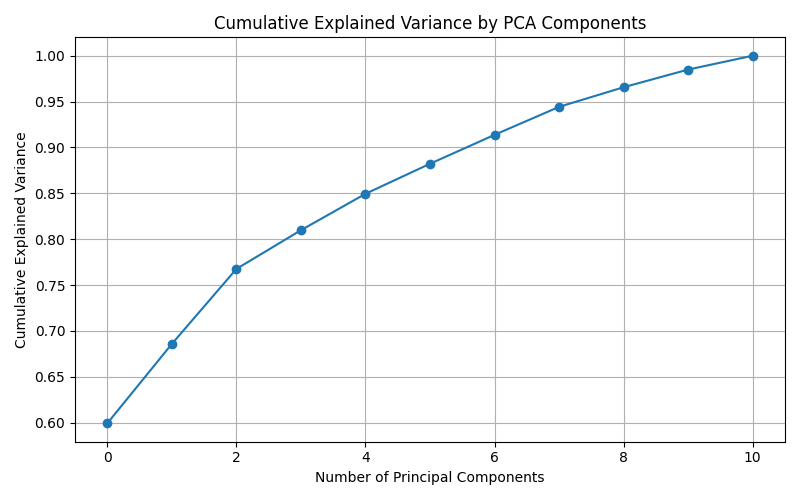
\includegraphics[width=\textwidth]{figures/pca_explained_variance.png}
        \caption{Cumulative explained variance by number of principal components.}
        \label{A}
    \end{minipage}
    \hfill
    \begin{minipage}[t]{0.48\textwidth}
        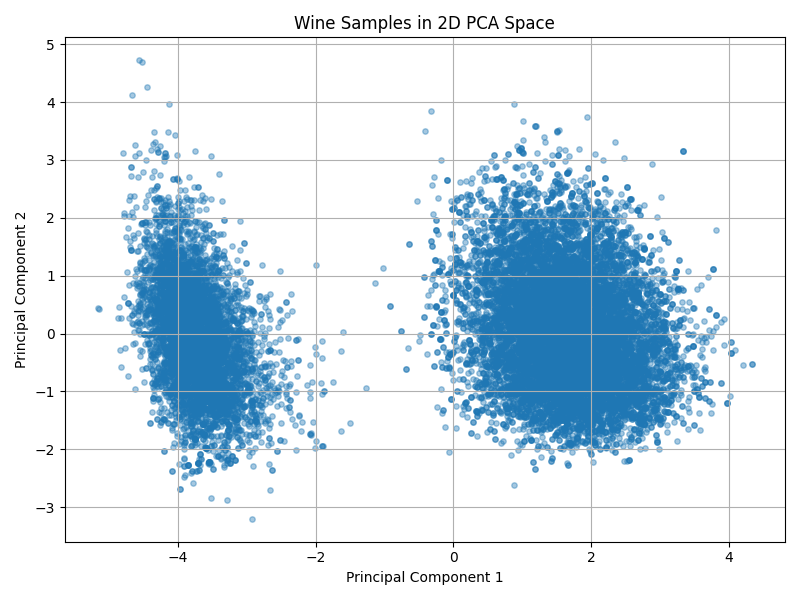
\includegraphics[width=\textwidth]{figures/pca_scatter_plot.png}
        \caption{2D PCA scatter plot of wine samples in the first two components.}
        \label{B}
    \end{minipage}
\end{figure}

\begin{figure}[H]
    \centering
    \begin{minipage}[t]{0.48\textwidth}
        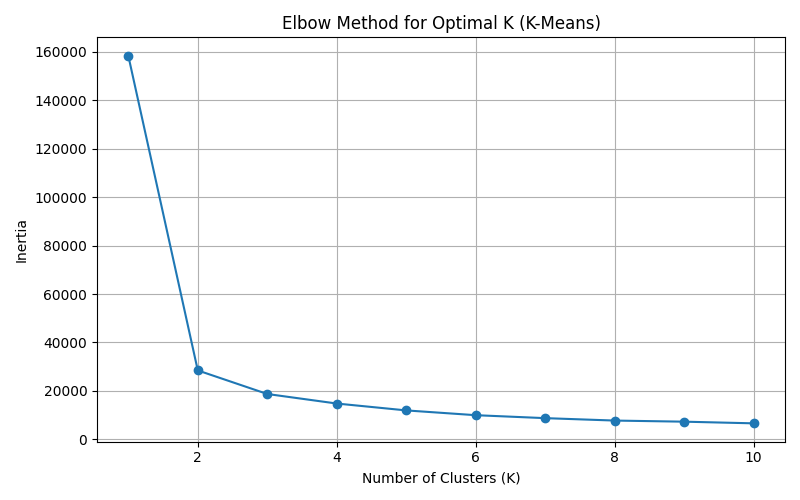
\includegraphics[width=\textwidth]{figures/kmeans_elbow.png}
        \caption{Elbow method for determining optimal $K$ in K-Means ($K=3$).}
        \label{C}
    \end{minipage}
    \hfill
    \begin{minipage}[t]{0.48\textwidth}
        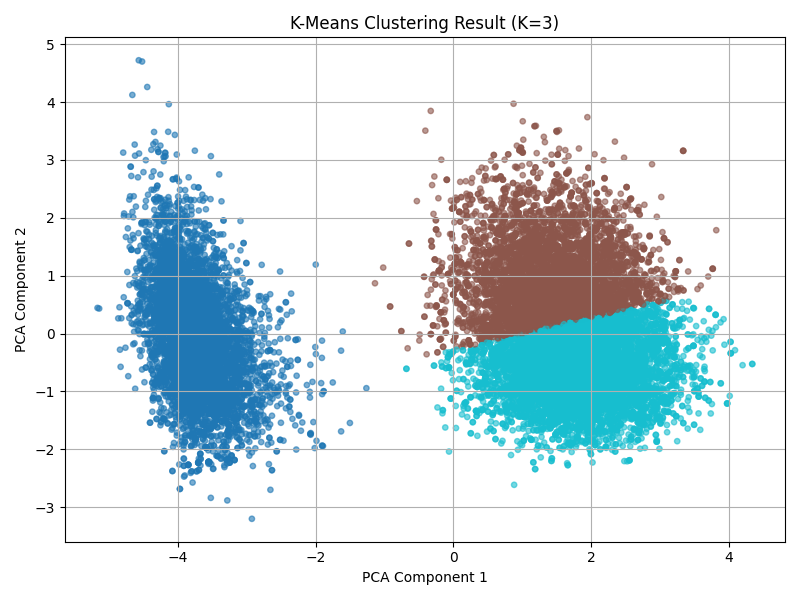
\includegraphics[width=\textwidth]{figures/kmeans_clustered_pca_k3.png}
        \caption{K-Means clustering result with $K=3$ in PCA space.}
        \label{D}
    \end{minipage}
\end{figure}

\begin{figure}[H]
    \centering
    \begin{minipage}[t]{0.48\textwidth}
        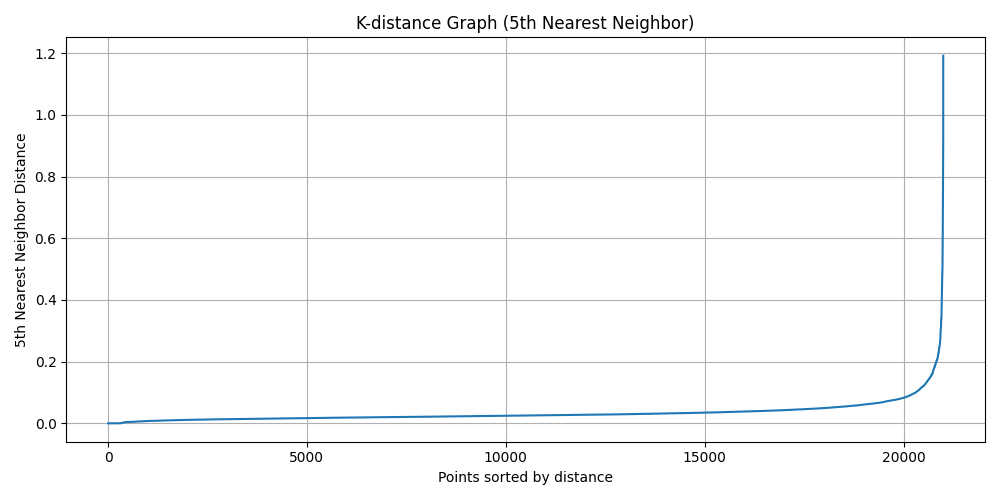
\includegraphics[width=\textwidth]{figures/dbscan_k_distance_explained.png}
        \caption{K-distance graph for selecting $\epsilon$ in DBSCAN.}
        \label{E}
    \end{minipage}
    \hfill
    \begin{minipage}[t]{0.48\textwidth}
        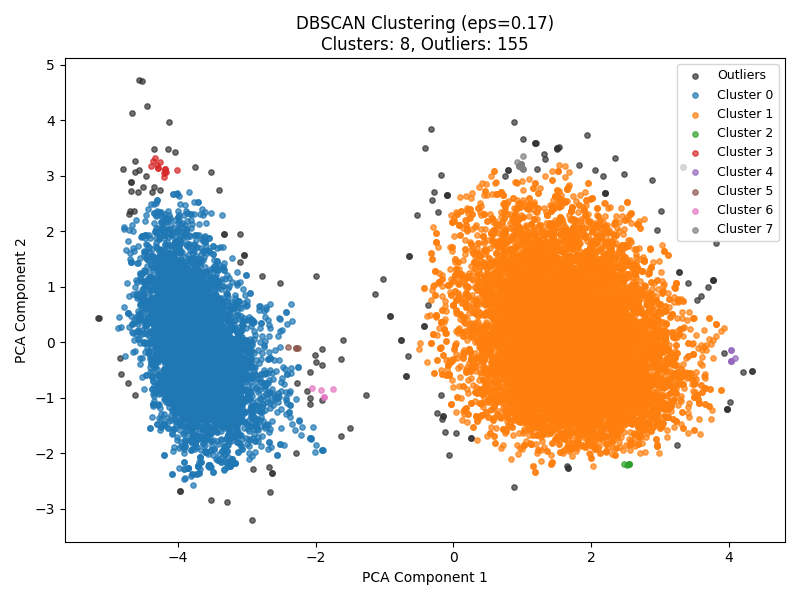
\includegraphics[width=\textwidth]{figures/dbscan_result_explained.png}
        \caption{DBSCAN result with 155 outliers shown in gray.}
        \label{F}
    \end{minipage}
\end{figure}

\begin{figure}[H]
    \centering
    \begin{minipage}[t]{0.48\textwidth}
        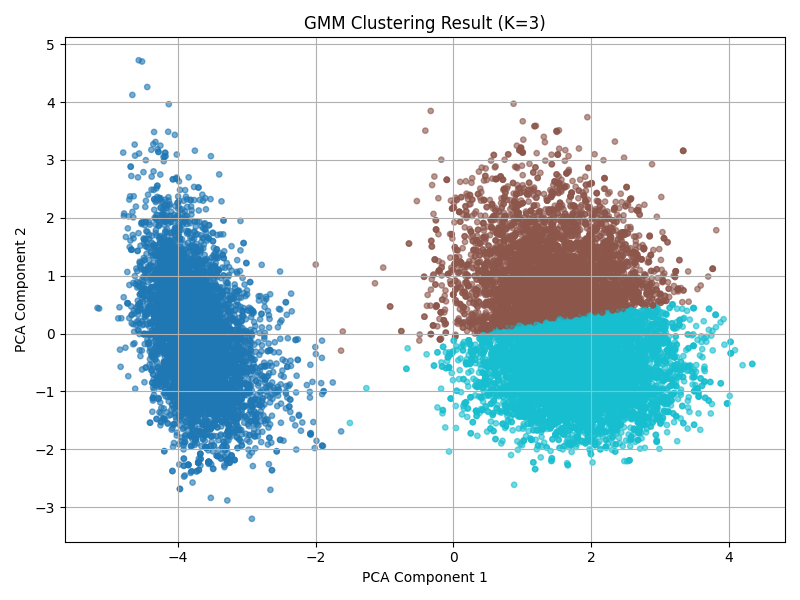
\includegraphics[width=\textwidth]{figures/gmm_clustered_pca_k3.png}
        \caption{GMM clustering with $K=3$ in PCA space (soft assignments).}
        \label{G}
    \end{minipage}
    \hfill
    \begin{minipage}[t]{0.48\textwidth}
        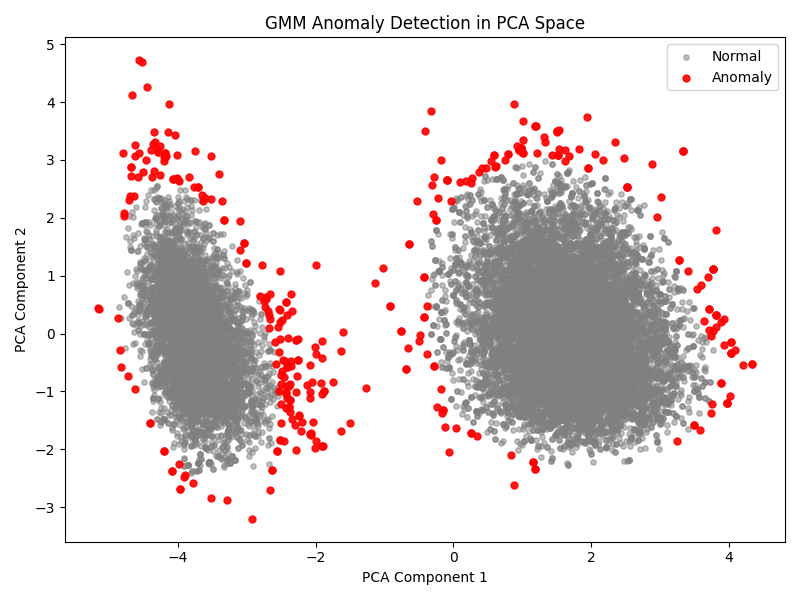
\includegraphics[width=\textwidth]{figures/gmm_anomaly_scatter.png}
        \caption{GMM anomaly detection: outliers in red (low log-likelihood).}
        \label{I}
    \end{minipage}
\end{figure}

\begin{figure}[H]
    \centering
    \begin{minipage}[t]{0.48\textwidth}
        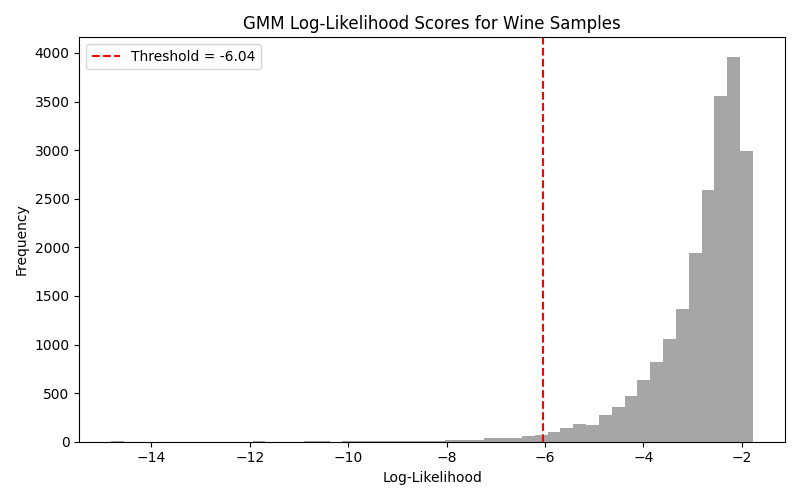
\includegraphics[width=\textwidth]{figures/gmm_anomaly_score_hist.png}
        \caption{Histogram of GMM log-likelihood scores. Red line shows anomaly threshold.}
        \label{H}
    \end{minipage}
    \hfill
    \begin{minipage}[t]{0.48\textwidth}
        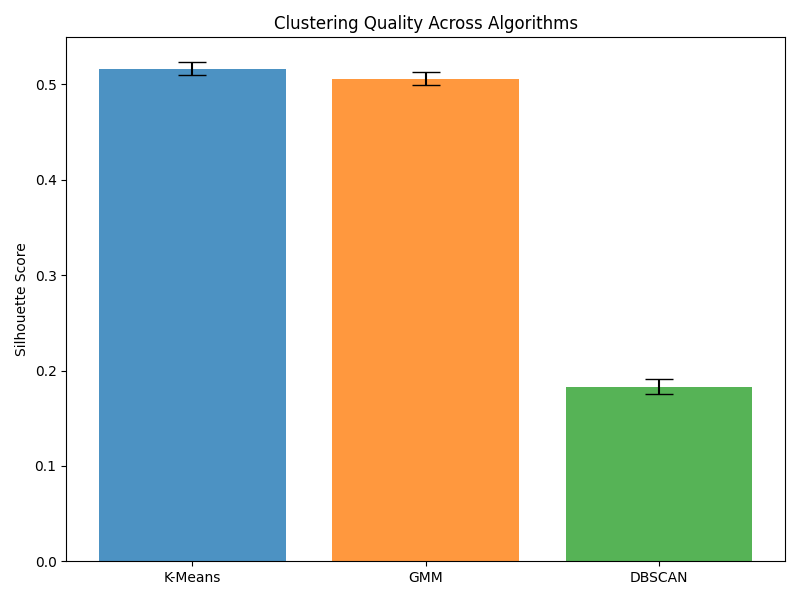
\includegraphics[width=\textwidth]{figures/silhouette_barplot.png}
        \caption{Silhouette scores across algorithms with standard deviation.}
        \label{J}
    \end{minipage}
\end{figure}

\begin{figure}[H]
    \centering
    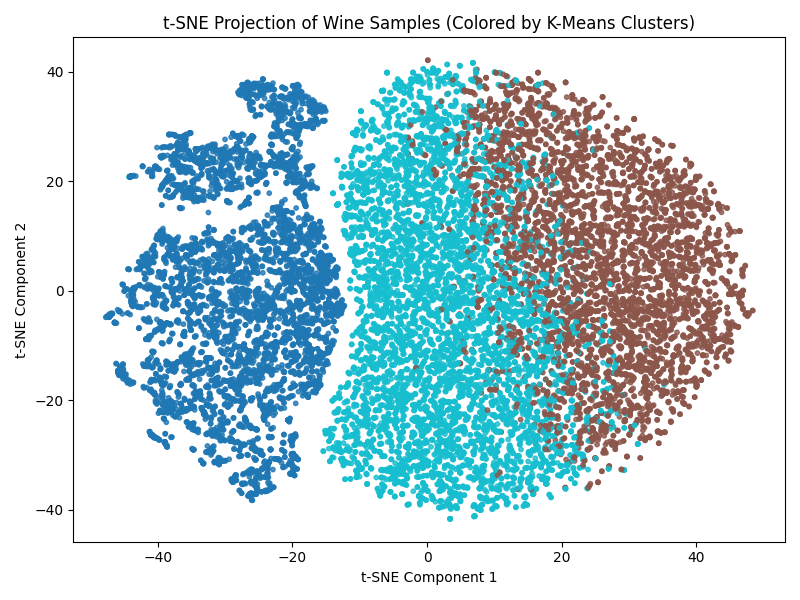
\includegraphics[width=0.6\textwidth]{figures/tsne_kmeans.png}
    \caption{t-SNE projection of wine samples colored by K-Means cluster labels.}
    \label{L}
\end{figure}



\section{Discussion}

In this project, we explored the latent structure of a wine dataset using a diverse set of unsupervised learning techniques. By applying dimensionality reduction, clustering, and anomaly detection methods, we uncovered meaningful patterns and subgroups based solely on the wines' chemical compositions — without using any target labels or quality scores. Each claim was backed by statistical evaluation or visual evidence, contributing to a comprehensive analysis pipeline.

Among the clustering algorithms, both K-Means and Gaussian Mixture Models (GMM) produced similarly high silhouette scores ($\approx$ 0.51), and both revealed three compact, well-separated clusters in PCA and t-SNE visualizations. K-Means provided simple, interpretable partitions, while GMM offered a probabilistic view with soft assignments. In contrast, DBSCAN discovered more complex structures and flagged 155 density-based outliers. Its lower silhouette score (0.18) reflects its ability to find non-convex clusters, but also its sensitivity to parameter choice and density variation. The combination of linear (K-Means, GMM) and density-based (DBSCAN) models provided complementary views of the data's geometry.

Anomaly detection yielded particularly interesting results. DBSCAN identified points in sparse regions, while GMM flagged 352 samples with unusually low log-likelihood under the model’s distribution. The two sets of outliers showed only partial overlap, indicating that each method captured different notions of “anomaly”: one based on spatial isolation, and the other based on statistical unlikelihood. These findings suggest that using multiple anomaly detectors in tandem can offer a more robust picture of rare or atypical samples in high-dimensional datasets.

Finally, the t-SNE visualization added interpretability by projecting the data into a non-linear 2D space. The K-Means clusters remained clearly distinguishable, reaffirming the effectiveness of the clustering. While PCA gave us variance-based structure, t-SNE helped reveal local neighborhoods and non-linear separation. This kind of visualization is invaluable for understanding the geometry of clustering results and can be extended to 3D or even interactive plots in future work. Other extensions might include feature attribution for cluster membership, deeper comparison with domain labels (e.g., wine type or origin), or training self-supervised models on this structure.

To better understand what distinguishes the discovered clusters, we analyzed the distribution of key features within each group. Cluster 0 showed significantly lower alcohol and sugar levels, suggesting these wines are lighter and milder. Cluster 1 had higher alcohol and pH, indicating stronger, drier wines with more preservatives. Cluster 2 displayed high acidity and low pH, which may be characteristic of sharper or longer-lasting wines. While we did not use labels or wine types in our analysis, these patterns suggest that the clustering captures real, interpretable wine styles. 

Beyond technical insights, these results could assist winemakers and wine retailers in understanding natural groupings of wines based on chemistry. For example, clustering can help segment wine styles for marketing, identify unexpected chemical profiles in production, or support quality control. The ability to detect outliers may flag rare or experimental batches, while visualizations such as t-SNE can aid in exploring product portfolios.


\section*{References}

\begin{thebibliography}{9}

\bibitem{murphy}
K. P. Murphy, \textit{Unsupervised Learning: Foundations of Clustering, Representation Learning, and Data Generation}. MIT Press, 2023.

\bibitem{tsne}
L. van der Maaten and G. Hinton, \textit{Visualizing Data using t-SNE}. Journal of Machine Learning Research, 9(Nov):2579–2605, 2008.

\bibitem{dbscan}
M. Ester, H.-P. Kriegel, J. Sander, and X. Xu, \textit{A Density-Based Algorithm for Discovering Clusters in Large Spatial Databases with Noise}. KDD, 1996.

\bibitem{gmm}
C. M. Bishop, \textit{Pattern Recognition and Machine Learning}. Springer, 2006.

\bibitem{scikit}
F. Pedregosa et al., \textit{Scikit-learn: Machine Learning in Python}. JMLR 12, pp. 2825–2830, 2011.

\bibitem{pandas}
W. McKinney, \textit{Data Structures for Statistical Computing in Python}. Proc. Python in Science Conf., 2010.

\bibitem{matplotlib}
J. D. Hunter, \textit{Matplotlib: A 2D Graphics Environment}. Computing in Science \& Engineering, 9(3):90–95, 2007.

\bibitem{kaggle}
T. Lo, \textit{Wine Quality Dataset (Balanced Classification)}. Kaggle. \url{https://www.kaggle.com/datasets/taweilo/wine-quality-dataset-balanced-classification}

\end{thebibliography}

\end{document}
